%========ANÁLISIS DEL SENSOR DE PULSO=======

\subsection{Sensor de pulso}
Para determinar el sensor de pulso, se realizó una tabla comparativa considerando diversos sensores de tipo fotopletismógrafos y ECG. \\

Las principales características a considerar para la selección del sensor fue el tipo, analógico o digital, y, en caso de ser digital, la resolución. Adicionalmente, se consideró la interfaz de comunicación que proporcionan, la cual será utilizada para realizar la comunicación con el microcontrolador.\\

En la Tabla \ref{analisis:sensorPulso} se muestran los datos de los diferentes sensores para cada característica.

	%\begin{sidewaystable}
\begin{table}[htbp]
	\begin{center}
		\scalebox{0.95}[0.95]{
		\begin{tabular}{|c|c|c|c|c|c|c|}
			\hline
			%			\rowcolor{colorSecundario}
			%			\color{green}
			\thead{Modelo}&\thead{Tipo}&\thead{Interfaz}&\thead{Resolución \\ (bits)}&\thead{Voltaje \\ (V)}& \thead{Corriente \\ (A)}&\thead{Precio\\ (USD)}\\
			\hline
			\hline
			PulseSensor & Analógico&-&-& 3.3 - 5&4m&24.99 \\
			\hline
			Finger Heart Rate Sensor & Analógico& -&- & 3.3 - 5&&0.74 \\
			\hline
			AD8232 & Analógico& -& - & 2 - 3.5&&29.5 \\
			\hline
			ADP103 & Digital& I2C& 14 & 1.7 - 1.9&$600\mu$&3 \\
			\hline
			MAX30100 & Digital& I2C &14 & 1.7 - 2&$600\mu$&14.99 \\
			\hline
		\end{tabular}}
		\caption{Comparativa de sensores de pulso.}
		\label{analisis:sensorPulso}
	\end{center}
\end{table}
	%\end{sidewaystable}	
Para el sensor de pulso se probarán dos sensores, uno de tipo ECG y otro PPG con el fin de comparar las señales entregadas y seleccionar la opción que mejor se comporte en mediciones sin una preparación tan estricta. \\

Debido a las características que presentan y que son sensores de uso común, se decidió utilizar el sensor \textbf{PulseSensor} y el \textbf{AD8232} mostrados en las figuras \ref{fig:AnalisispulseSensor} y \ref{fig:AnalisisAD8232}. \\

		\begin{figure}[htbp!]
			\centering
			\fbox{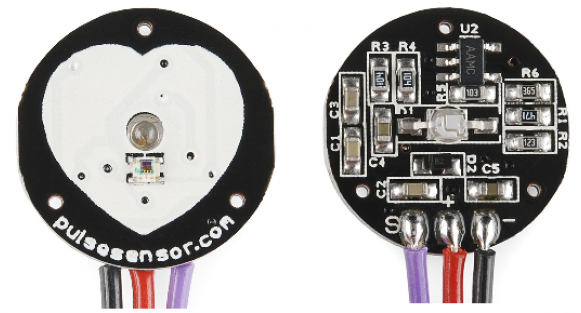
\includegraphics[width=0.4\textwidth]{Analisis/imagenes/pulsesensor.png}}
			\caption{Pulse Sensor.}
			\label{fig:AnalisispulseSensor}
		\end{figure}

		\begin{figure}[htbp!]
			\centering
			\fbox{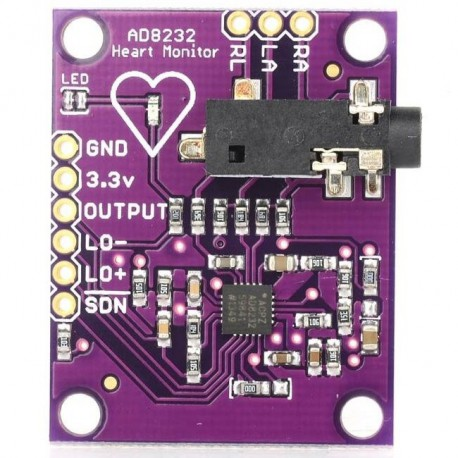
\includegraphics[width=0.35\textwidth]{Analisis/imagenes/ad8232.jpg}}
			\caption{AD8232}
			\label{fig:AnalisisAD8232}
		\end{figure}
\pagebreak